\documentclass[12pt,a4paper]{report}
\usepackage[utf8]{inputenc}
\usepackage[T1]{fontenc}
\usepackage{geometry}
\usepackage{setspace}
\usepackage{graphicx}
\usepackage{float}
\usepackage{array}
\usepackage{longtable}
\usepackage{booktabs}
\usepackage{titlesec}
\usepackage{hyperref}
\usepackage{enumitem}
\usepackage{fancyhdr}
\usepackage{color}
\usepackage{tikz}
\usetikzlibrary{shapes.geometric, arrows.meta, positioning}

\geometry{margin=1in}
\onehalfspacing
\setcounter{tocdepth}{2}

\hypersetup{
  colorlinks=true,
  linkcolor=blue,
  urlcolor=blue,
  pdftitle={Final Project Report - AI Chatbot with Resume Builder},
  pdfauthor={Amruta Anil Bargal, Prof. Dahane G.M.}
}

\pagestyle{fancy}
\fancyhf{}
\fancyhead[L]{AI Chatbot Final Project Report}
\fancyhead[R]{\thepage}

\newcommand{\screenshotplaceholder}[2]{
\begin{figure}[H]
\centering
\fbox{
\begin{minipage}[c][2.8in][c]{0.9\textwidth}
\centering
\textbf{#1}\\[8pt]
Insert screenshot file here\\
(#2)
\end{minipage}
}
\caption{#1}
\end{figure}
}

\begin{document}

% -------------------- TITLE PAGE --------------------
\begin{titlepage}
\centering
\vspace*{1cm}
{\Large \textbf{Dr. Vithalrao Vikhe Patil College Of Engineering, Ahmednagar}}\\[0.6cm]
{\large Department of Data Science Engineering}\\[1.6cm]

{\Huge \textbf{FINAL YEAR PROJECT REPORT}}\\[0.6cm]
{\Large on}\\[0.4cm]
{\LARGE \textbf{AI Chatbot with Resume Building:}}\\
{\LARGE \textbf{An Integrated Multi-Modal Conversational System}}\\[1.6cm]

\begin{tabular}{>{\bfseries}p{2.3in} p{3.0in}}
Submitted By: & Amruta Anil Bargal \\
Guide: & Prof. Dahane G.M. \\
Department: & Data Science Engineering \\
Academic Year: & 2025--2026 \\
\end{tabular}

\vfill
{\large Submitted in partial fulfillment of the requirements for the award of}\\
{\large \textbf{Bachelor of Engineering}}\\[0.8cm]
{\large \textbf{Savitribai Phule Pune University}}
\end{titlepage}

% -------------------- CERTIFICATE --------------------
\chapter*{Certificate}
\addcontentsline{toc}{chapter}{Certificate}
This is to certify that the project report entitled \textbf{``AI Chatbot with Resume Building: An Integrated Multi-Modal Conversational System''} is a bonafide work carried out by \textbf{Amruta Anil Bargal} under the guidance of \textbf{Prof. Dahane G.M.}, Department of Data Science Engineering, Dr. Vithalrao Vikhe Patil College Of Engineering, Ahmednagar, during the academic year 2025--2026.

\vspace{1.2in}
\noindent
\begin{tabular}{p{2.5in} p{2.5in}}
\textbf{Project Guide} & \textbf{Head of Department}\\
Prof. Dahane G.M. & Data Science Engineering
\end{tabular}

\vspace{0.8in}
\noindent\textbf{Principal}

% -------------------- DECLARATION --------------------
\chapter*{Declaration}
\addcontentsline{toc}{chapter}{Declaration}
I hereby declare that the project work presented in this report is my original work and has been carried out by me under the supervision of \textbf{Prof. Dahane G.M.}. This report has not been submitted in full or in part for any other degree or diploma.

\vspace{1in}
\noindent
\textbf{Amruta Anil Bargal}\\
Department of Data Science Engineering

% -------------------- ACK --------------------
\chapter*{Acknowledgment}
\addcontentsline{toc}{chapter}{Acknowledgment}
I express my sincere gratitude to \textbf{Prof. Dahane G.M.} for valuable guidance, constant support, and motivation throughout this project. I also thank the Department of Data Science Engineering and Dr. Vithalrao Vikhe Patil College Of Engineering, Ahmednagar, for providing the infrastructure and academic environment necessary to complete this work.

% -------------------- ABSTRACT --------------------
\chapter*{Abstract}
\addcontentsline{toc}{chapter}{Abstract}
This project presents an integrated web-based AI chatbot platform combining conversational intelligence, multi-modal file understanding, and ATS-aware resume generation. The system supports text, image, video, and PDF processing; real-time chat interactions; voice input; and career-document assistance. The architecture is modular and scalable, built with modern frontend technologies and AI APIs. The implemented system includes chat history management, export mechanisms, search functionality, and a resume builder with template-driven output and AI-assisted content suggestions. Evaluation indicates practical usability for students and job seekers while highlighting scope for enhancement in areas such as collaboration, advanced analytics, and stronger privacy controls.

\tableofcontents
\listoffigures
\listoftables
\clearpage

% ==================== CHAPTER 1 ====================
\chapter{Introduction}
\section{Project Background}
Artificial Intelligence has transformed human-computer interaction from command-based interfaces to contextual, conversational systems. Chatbots today are used in customer support, education, productivity, healthcare triage, and professional assistance. In parallel, recruitment ecosystems now rely heavily on Applicant Tracking Systems (ATS), which parse and rank resumes before human review. This shift has created a need for tools that help candidates prepare structured, keyword-aligned, and readable resumes.

\section{Problem Statement}
Most existing tools are fragmented:
\begin{itemize}
  \item conversational assistants are separate from resume platforms,
  \item file understanding tools are disconnected from career guidance,
  \item ATS checks and content generation are often isolated utilities.
\end{itemize}
This fragmentation causes repeated context switching, reduced productivity, and inconsistent document quality.

\section{Project Objectives}
\begin{enumerate}
  \item Build a conversational AI assistant for real-time multi-turn support.
  \item Enable multi-modal file processing (text, image, video, PDF).
  \item Integrate resume generation with ATS-oriented recommendations.
  \item Provide practical utilities: search, save/load, export, and voice input.
  \item Design a modular architecture that is easy to maintain and extend.
\end{enumerate}

\section{Scope}
The project scope includes client-side interaction, API-based AI responses, resume content generation, and user-oriented productivity features. The current scope excludes enterprise SSO, production-grade encryption infrastructure, and large-scale cloud orchestration.

\section{Report Organization}
This report is organized into chapters covering literature review, requirement analysis, system design, implementation, testing, results, limitations, and future work with appendices for screenshots and technical artifacts.

% ==================== CHAPTER 2 ====================
\chapter{Literature Review}
\section{Evolution of Chatbot Systems}
From ELIZA-style pattern matching to modern transformer-based models, chatbot systems have evolved significantly in language understanding and response quality. Rule-based systems are predictable but rigid; LLM-based systems are fluent but probabilistic.

\section{Multi-Modal AI in Practical Applications}
Recent research emphasizes multimodal processing where models combine textual and visual/document signals to improve contextual understanding. This is especially important in workflows where users upload resumes, job descriptions, or project files.

\section{Voice Interfaces and Accessibility}
Browser-based speech APIs have increased accessibility for users with typing constraints and have improved interaction speed for ideation tasks.

\section{Resume Intelligence and ATS Compatibility}
ATS-oriented resume systems have emerged as a focused application area. They improve formatting and keyword alignment but often lack iterative conversational guidance.

\section{Research Gap}
A common gap identified in literature is the absence of unified platforms combining conversational context, multimodal document understanding, and ATS-aware resume generation in one coherent user experience.

% ==================== CHAPTER 3 ====================
\chapter{Requirement Analysis}
\section{Functional Requirements}
\begin{itemize}
  \item User chat input and AI response generation.
  \item File upload and parsing for supported formats.
  \item Voice input for prompt creation.
  \item Chat history persistence and retrieval.
  \item Resume generation with templates and AI content support.
  \item Export to multiple formats (text, PDF, JSON).
\end{itemize}

\section{Non-Functional Requirements}
\begin{itemize}
  \item Usability: clean interface with minimal friction.
  \item Performance: low-latency interaction for normal workloads.
  \item Reliability: graceful handling of API or network failures.
  \item Maintainability: modular and readable code organization.
  \item Portability: browser compatibility across major environments.
\end{itemize}

\section{Software and Hardware Requirements}
\begin{table}[H]
\centering
\caption{System Requirements}
\begin{tabular}{|p{1.7in}|p{3.4in}|}
\hline
\textbf{Component} & \textbf{Requirement} \\
\hline
Operating System & Windows / Linux / macOS \\
\hline
Browser & Chrome / Edge / Firefox (modern versions) \\
\hline
Runtime & Node.js (for server version) \\
\hline
Frontend & HTML5, CSS3, JavaScript (ES6+) \\
\hline
AI Services & Gemini/Groq API, optional Hugging Face \\
\hline
Storage & Browser localStorage \\
\hline
\end{tabular}
\end{table}

% ==================== CHAPTER 4 ====================
\chapter{System Analysis and Design}
\section{Overall Architecture}
The architecture follows layered modular design:
\begin{enumerate}
  \item Presentation Layer (UI components, forms, modals, visual feedback)
  \item Processing Layer (prompt handling, file parsing, validation)
  \item AI Integration Layer (API request/response orchestration)
  \item Persistence Layer (history save/load, export state, session context)
\end{enumerate}

\section{Architecture Diagram}
\begin{figure}[H]
\centering
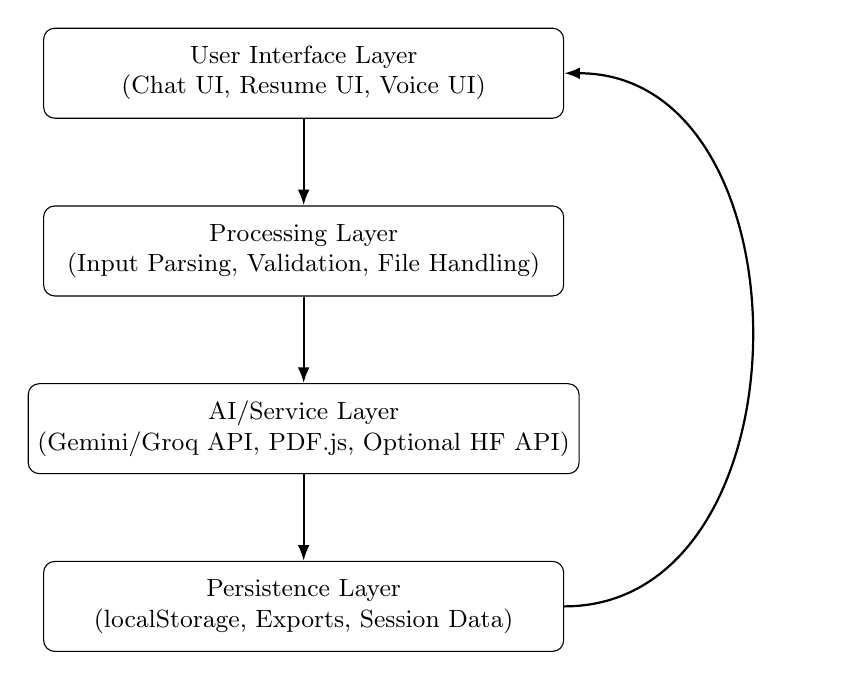
\begin{tikzpicture}[
  node distance=1.1cm and 1.2cm,
  every node/.style={font=\small},
  box/.style={rectangle, draw, rounded corners, minimum width=2.6in, minimum height=0.45in, align=center},
  arr/.style={-{Latex[length=2mm]}, thick}
]
\node[box] (ui) {User Interface Layer\\(Chat UI, Resume UI, Voice UI)};
\node[box, below=of ui] (proc) {Processing Layer\\(Input Parsing, Validation, File Handling)};
\node[box, below=of proc] (api) {AI/Service Layer\\(Gemini/Groq API, PDF.js, Optional HF API)};
\node[box, below=of api] (store) {Persistence Layer\\(localStorage, Exports, Session Data)};
\draw[arr] (ui) -- (proc);
\draw[arr] (proc) -- (api);
\draw[arr] (api) -- (store);
\draw[arr] (store.east) to[out=0,in=0,looseness=1.2] (ui.east);
\end{tikzpicture}
\caption{Layered System Architecture}
\end{figure}

\section{Flowchart: Chat Request Lifecycle}
\begin{figure}[H]
\centering
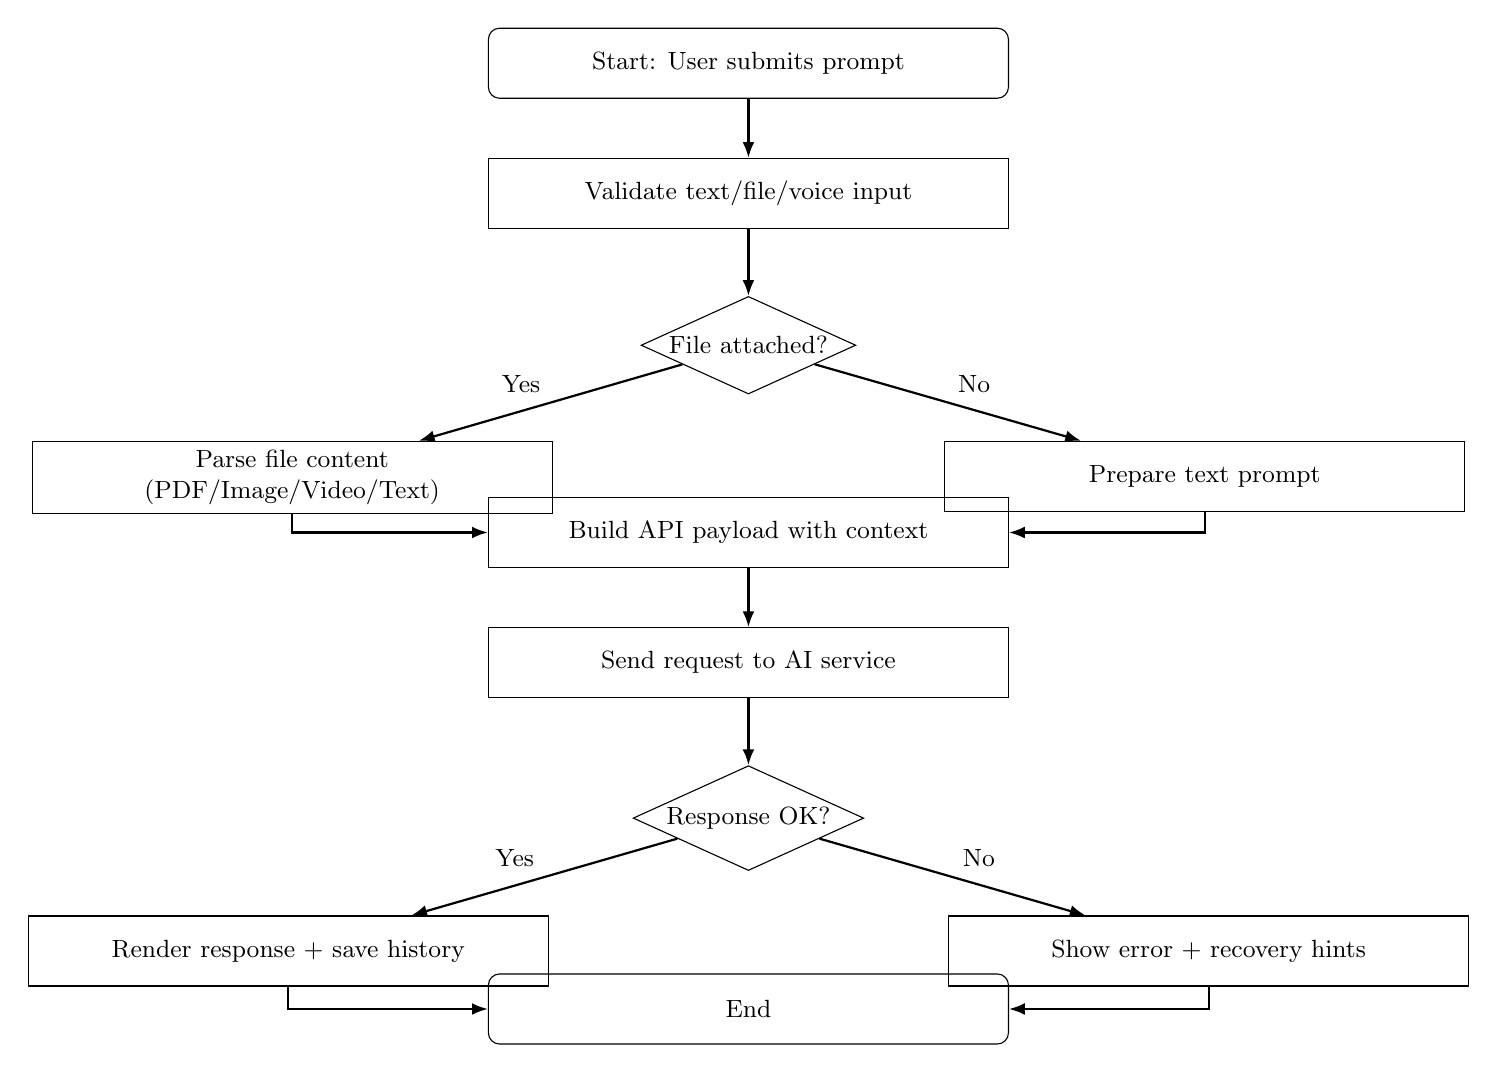
\begin{tikzpicture}[
  node distance=0.75cm,
  startstop/.style={rectangle, rounded corners, draw, minimum width=2.6in, minimum height=0.35in, align=center},
  process/.style={rectangle, draw, minimum width=2.6in, minimum height=0.35in, align=center},
  decision/.style={diamond, draw, aspect=2.2, align=center, inner sep=1pt},
  arr/.style={-{Latex[length=2mm]}, thick},
  font=\small
]
\node[startstop] (start) {Start: User submits prompt};
\node[process, below=of start] (validate) {Validate text/file/voice input};
\node[decision, below=of validate, yshift=-0.1cm] (filecheck) {File attached?};
\node[process, below left=0.9cm and 1.8cm of filecheck] (parse) {Parse file content\\(PDF/Image/Video/Text)};
\node[process, below right=0.9cm and 1.8cm of filecheck] (textonly) {Prepare text prompt};
\node[process, below=1.3cm of filecheck] (payload) {Build API payload with context};
\node[process, below=of payload] (send) {Send request to AI service};
\node[decision, below=of send, yshift=-0.1cm] (ok) {Response OK?};
\node[process, below left=0.9cm and 1.8cm of ok] (render) {Render response + save history};
\node[process, below right=0.9cm and 1.8cm of ok] (error) {Show error + recovery hints};
\node[startstop, below=1.3cm of ok] (end) {End};
\draw[arr] (start) -- (validate);
\draw[arr] (validate) -- (filecheck);
\draw[arr] (filecheck) -- node[above left]{Yes} (parse);
\draw[arr] (filecheck) -- node[above right]{No} (textonly);
\draw[arr] (parse) |- (payload);
\draw[arr] (textonly) |- (payload);
\draw[arr] (payload) -- (send);
\draw[arr] (send) -- (ok);
\draw[arr] (ok) -- node[above left]{Yes} (render);
\draw[arr] (ok) -- node[above right]{No} (error);
\draw[arr] (render) |- (end);
\draw[arr] (error) |- (end);
\end{tikzpicture}
\caption{Chat Processing Flowchart}
\end{figure}

\section{Data Flow Description}
Input data enters from text, voice, or file upload. The system validates and normalizes data, constructs model-compatible payloads, dispatches requests to AI endpoints, and renders responses with typing effects. Relevant state is persisted for continuity and export.

\section{Subsystem Architecture Details}
\subsection{Frontend Subsystem}
The frontend subsystem is responsible for rendering chat messages, handling user actions, and maintaining responsive interaction states. It includes:
\begin{itemize}
  \item prompt input and validation handlers,
  \item dynamic message rendering with typing simulation,
  \item modal components for resume builder and export tools,
  \item theme switching and accessibility-oriented controls.
\end{itemize}

\subsection{AI Service Subsystem}
This subsystem handles model communication and response control:
\begin{itemize}
  \item building request payloads from text and file context,
  \item sending API calls and parsing structured responses,
  \item retry/failure handling for transient network issues,
  \item response post-processing for UI-safe rendering.
\end{itemize}

\subsection{Persistence Subsystem}
Persistence utilities preserve continuity and reduce user effort:
\begin{itemize}
  \item browser localStorage for session state,
  \item chat save/load and data export utilities,
  \item safe reset and cleanup utilities for corrupted states.
\end{itemize}

\section{Deployment View}
\begin{figure}[H]
\centering
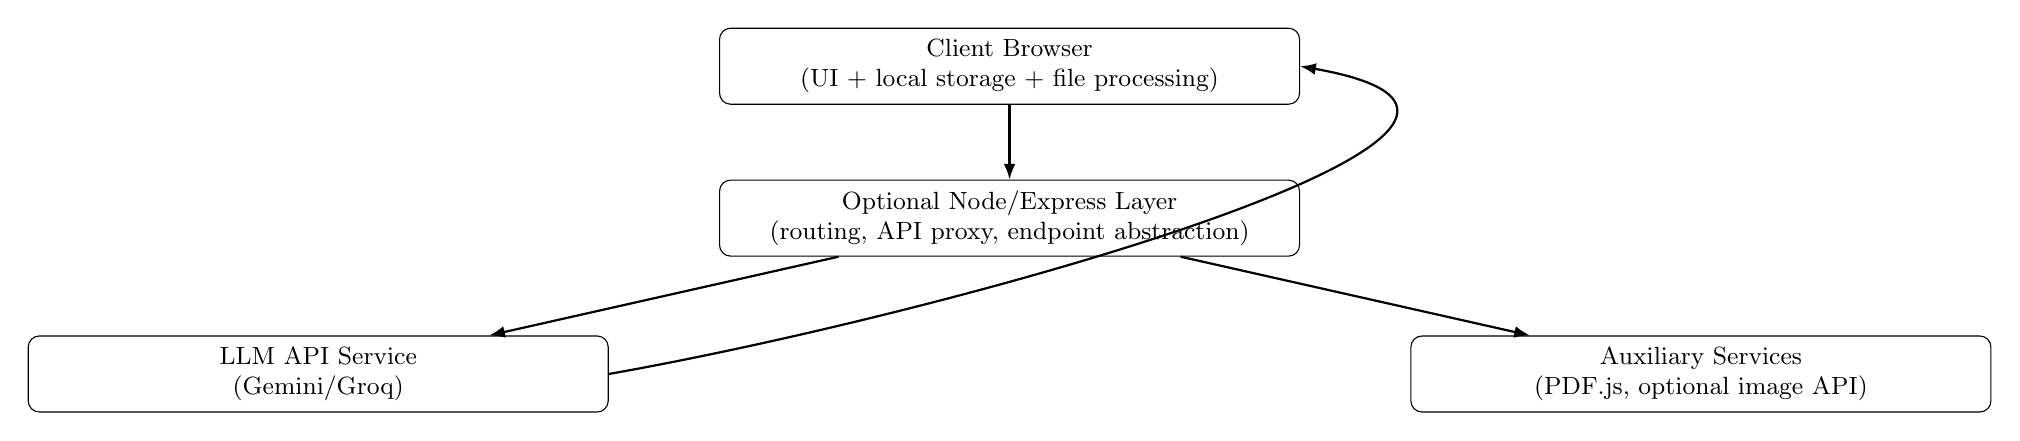
\begin{tikzpicture}[
  node distance=0.95cm,
  box/.style={rectangle, draw, rounded corners, minimum width=2.9in, minimum height=0.38in, align=center},
  arr/.style={-{Latex[length=2mm]}, thick},
  font=\small
]
\node[box] (client) {Client Browser\\(UI + local storage + file processing)};
\node[box, below=of client] (server) {Optional Node/Express Layer\\(routing, API proxy, endpoint abstraction)};
\node[box, below left=1.0cm and 1.4cm of server] (llm) {LLM API Service\\(Gemini/Groq)};
\node[box, below right=1.0cm and 1.4cm of server] (aux) {Auxiliary Services\\(PDF.js, optional image API)};
\draw[arr] (client) -- (server);
\draw[arr] (server) -- (llm);
\draw[arr] (server) -- (aux);
\draw[arr] (llm.east) to[out=10,in=350,looseness=1.15] (client.east);
\end{tikzpicture}
\caption{Deployment-Level View}
\end{figure}

% ==================== CHAPTER 5 ====================
\chapter{Software Tools and Development Environment}
\section{Development Tools}
\begin{table}[H]
\centering
\caption{Software Tools Used}
\begin{tabular}{|p{2.2in}|p{2.3in}|}
\hline
\textbf{Tool/Platform} & \textbf{Purpose} \\
\hline
Visual Studio Code / Cursor IDE & Development and debugging \\
\hline
Node.js and npm & Runtime and package management \\
\hline
Git and GitHub & Version control and collaboration \\
\hline
Chrome/Edge DevTools & Client-side debugging and profiling \\
\hline
PDF.js & Client-side PDF text extraction \\
\hline
html2pdf.js & Document export to PDF \\
\hline
\end{tabular}
\end{table}

\section{APIs and External Services}
\begin{itemize}
  \item \textbf{Generative AI API:} conversational responses and content generation.
  \item \textbf{Speech API:} voice-to-text prompt creation.
  \item \textbf{Optional image API:} media-generation support for extended modules.
\end{itemize}

\section{Configuration and Environment Variables}
For secure deployment, keys and service settings should be configured through environment variables rather than hard-coded values. Recommended variables include:
\begin{itemize}
  \item \texttt{GROQ\_API\_KEY} or equivalent LLM key,
  \item \texttt{HUGGINGFACE\_API\_KEY} (optional),
  \item \texttt{PORT} for local/hosted runtime.
\end{itemize}

\section{Build and Run Workflow}
\begin{enumerate}
  \item Install dependencies with package manager.
  \item Configure environment file with keys.
  \item Start local server/runtime.
  \item Validate health endpoint and UI load.
  \item Run module-wise manual test checklist.
\end{enumerate}

\section{Development Standards Followed}
\begin{itemize}
  \item modular separation of concerns,
  \item clear naming for UI handlers and service functions,
  \item explicit error handling and fallback messaging,
  \item reusable utility methods for parsing/export flows.
\end{itemize}

% ==================== CHAPTER 6 ====================
\chapter{Implementation Details}
\section{Technology Stack}
\begin{itemize}
  \item Frontend: HTML5, CSS3, JavaScript (Vanilla ES6+)
  \item APIs: Gemini/Groq chat APIs, optional Hugging Face image API
  \item Libraries: PDF.js, html2pdf.js
  \item Storage: Browser localStorage
  \item Optional backend: Node.js + Express
\end{itemize}

\section{Module-Wise Implementation}
\subsection{Chat Module}
Implements prompt handling, contextual history, response rendering, interruption controls, and copy/search utilities.

\subsection{File Processing Module}
Handles MIME detection and format-specific processing:
\begin{itemize}
  \item PDF text extraction,
  \item image/video inline processing,
  \item text and CSV reading,
  \item preview and cancellation.
\end{itemize}

\subsection{Voice Module}
Uses browser speech recognition APIs for real-time transcription and user feedback animations.

\subsection{Resume Builder Module}
Provides template-based resume generation with AI-assisted summary and skills, ATS suggestions, and print/export support.

\subsection{Export and Persistence Module}
Supports autosave, session reload, JSON export/import, and PDF/text chat export.

\section{Pseudo Algorithms}
\subsection{Typing Effect}
\begin{enumerate}
  \item Split model response into word array.
  \item Append one word per interval.
  \item Auto-scroll and finalize state.
  \item Persist updated chat state.
\end{enumerate}

\subsection{ATS Keyword Support}
\begin{enumerate}
  \item Parse role title and user experience blocks.
  \item Generate or suggest role-aligned skill set.
  \item Highlight missing common ATS terms.
  \item Regenerate sections with balanced readability.
\end{enumerate}

% ==================== CHAPTER 7 ====================
\chapter{Screenshots and UI Walkthrough}
\section{Main Chat Interface}
\screenshotplaceholder{Main Dashboard / Chat Screen}{Home page with input panel, suggestions, and chat container}

\section{File Upload and Preview}
\screenshotplaceholder{File Upload Workflow}{User attaching PDF/image/video and preview before sending}

\section{Voice Input Module}
\screenshotplaceholder{Voice Recognition View}{Microphone active state and transcription behavior}

\section{Search and Chat History}
\screenshotplaceholder{History and Search Feature}{Search in previous conversation and highlight results}

\section{Resume Builder Form}
\screenshotplaceholder{Resume Builder Input Form}{Personal details, education, experience, skills}

\section{Resume Template Preview}
\screenshotplaceholder{Resume Output Preview}{Template render output with ATS-oriented structure}

\section{Export Options}
\screenshotplaceholder{Export Modal}{Export chat/report into PDF, text, JSON}

\section{Theme and Settings}
\screenshotplaceholder{Theme Toggle and UI Preferences}{Light/Dark mode and configuration controls}

\section{Error Handling Screens}
\screenshotplaceholder{Error and Retry Feedback}{API/network error states with user-friendly messages}

\section{Mobile Responsive Layout}
\screenshotplaceholder{Responsive UI (Mobile View)}{App behavior on smaller screens}

% ==================== CHAPTER 8 ====================
\chapter{Testing and Validation}
\section{Testing Strategy}
\begin{itemize}
  \item Unit-level function verification for parser and utility functions.
  \item Integration testing for UI + API interactions.
  \item Usability testing with representative student users.
  \item Cross-browser compatibility validation.
\end{itemize}

\section{Test Cases}
\begin{longtable}{|p{0.8in}|p{2.2in}|p{1.0in}|p{1.3in}|}
\hline
\textbf{TC ID} & \textbf{Test Scenario} & \textbf{Expected} & \textbf{Result} \\
\hline
TC-01 & Send text query & Valid AI response & Pass \\
\hline
TC-02 & Upload PDF and ask summary & PDF text extracted and used & Pass \\
\hline
TC-03 & Upload unsupported file & Proper validation error & Pass \\
\hline
TC-04 & Voice to text prompt & Prompt transcribed correctly & Pass \\
\hline
TC-05 & Save and reload chat session & Session restored & Pass \\
\hline
TC-06 & Export chat as PDF & File generated & Pass \\
\hline
TC-07 & Resume generate from form & Rendered template output & Pass \\
\hline
TC-08 & ATS suggestion trigger & Skill/keyword advice shown & Pass \\
\hline
TC-09 & Search in long chat & Accurate highlights & Pass \\
\hline
TC-10 & API failure simulation & Graceful error feedback & Pass \\
\hline
\end{longtable}

\section{Performance Snapshot}
\begin{table}[H]
\centering
\caption{Observed Performance (Typical Conditions)}
\begin{tabular}{|p{2.4in}|p{2.3in}|}
\hline
\textbf{Metric} & \textbf{Observation} \\
\hline
Average AI response time & 2--5 seconds \\
\hline
PDF extraction time (normal file) & 1--3 seconds \\
\hline
Search latency (local history) & $<$100 ms (typical) \\
\hline
UI interaction smoothness & Stable (desktop modern browsers) \\
\hline
\end{tabular}
\end{table}

% ==================== CHAPTER 9 ====================
\chapter{Results and Discussion}
\section{Functional Outcomes}
The system successfully demonstrates integrated conversational support with multimodal file processing and resume generation. User experience is improved by consolidated workflow, reducing the need to switch between disconnected tools.

\section{Usability Insights}
Users benefit most from:
\begin{itemize}
  \item rapid drafting and rewriting support,
  \item contextual continuity in chat sessions,
  \item integrated resume and ATS guidance.
\end{itemize}

\section{Limitations}
\begin{itemize}
  \item API dependency and quota constraints,
  \item limited offline functionality,
  \item potential variability in model responses,
  \item browser-dependent voice behavior.
\end{itemize}

\section{Risk and Mitigation}
\begin{table}[H]
\centering
\caption{Risk Register}
\begin{tabular}{|p{1.6in}|p{1.2in}|p{2.2in}|}
\hline
\textbf{Risk} & \textbf{Impact} & \textbf{Mitigation} \\
\hline
API downtime & High & Retry logic + fallback messages \\
\hline
Quota exceeded & Medium & Key rotation guidance + usage alerts \\
\hline
Large file failure & Medium & Size validation + preprocessing hints \\
\hline
Incorrect AI output & High & User verification disclaimer + edit tools \\
\hline
\end{tabular}
\end{table}

% ==================== CHAPTER 10 ====================
\chapter{Project Management and Planning}
\section{Development Phases}
\begin{enumerate}
  \item Requirement analysis and feasibility.
  \item UI prototype and architecture setup.
  \item Core chatbot integration.
  \item Multi-modal processing implementation.
  \item Resume builder and ATS module.
  \item Testing, fixes, and documentation.
\end{enumerate}

\section{Timeline (Indicative)}
\begin{table}[H]
\centering
\caption{Phase Timeline}
\begin{tabular}{|p{2.6in}|p{1.8in}|}
\hline
\textbf{Phase} & \textbf{Duration} \\
\hline
Planning and Literature Review & 2--3 weeks \\
\hline
System Design & 2 weeks \\
\hline
Core Development & 5--6 weeks \\
\hline
Testing and Refinement & 2--3 weeks \\
\hline
Report and Finalization & 2 weeks \\
\hline
\end{tabular}
\end{table}

\section{Effort Distribution}
\begin{itemize}
  \item Design and Architecture: 20\%
  \item Development: 45\%
  \item Testing and Debugging: 20\%
  \item Documentation and Presentation: 15\%
\end{itemize}

% ==================== CHAPTER 11 ====================
\chapter{Detailed Analysis and Extended Data}
\section{Feature Inventory and Coverage}
The implemented system includes multiple major capability groups. Table \ref{tab:feature_inventory} summarizes category-wise coverage and implementation maturity.

\begin{table}[H]
\centering
\caption{Feature Inventory}
\label{tab:feature_inventory}
\begin{tabular}{|p{2.1in}|p{1.0in}|p{1.3in}|}
\hline
\textbf{Feature Category} & \textbf{Count} & \textbf{Status} \\
\hline
Core chat interaction & 8 & Implemented \\
\hline
Multi-modal file handling & 7 & Implemented \\
\hline
Chat history/search/export & 9 & Implemented \\
\hline
Voice input capabilities & 4 & Implemented \\
\hline
Resume builder modules & 12 & Implemented \\
\hline
UI/UX enhancements & 8 & Implemented \\
\hline
Advanced control features & 6 & Implemented \\
\hline
\end{tabular}
\end{table}

\section{Module Interaction Matrix}
The modules are tightly integrated but loosely coupled at implementation boundaries. Table \ref{tab:interaction_matrix} shows principal interactions.

\begin{table}[H]
\centering
\caption{Module Interaction Matrix}
\label{tab:interaction_matrix}
\begin{tabular}{|p{1.6in}|p{1.6in}|p{1.6in}|}
\hline
\textbf{Source Module} & \textbf{Target Module} & \textbf{Interaction Purpose} \\
\hline
Prompt Manager & API Gateway & Request dispatch and response handling \\
\hline
File Handler & Prompt Manager & Context augmentation from files \\
\hline
Voice Input & Prompt Manager & Transcription-to-prompt conversion \\
\hline
Resume Engine & AI Service Layer & Summary and skill generation \\
\hline
History Manager & Export Manager & Save/load/export orchestration \\
\hline
UI Renderer & History Manager & Display-state persistence \\
\hline
\end{tabular}
\end{table}

\section{Data Structures Used}
The implementation primarily uses lightweight in-memory and browser-native structures:
\begin{itemize}
  \item \textbf{Message Array:} stores ordered conversation objects (role, parts, timestamp).
  \item \textbf{Session Metadata Object:} stores preferences, active mode, template details.
  \item \textbf{File Descriptor Object:} stores MIME type, base64 payload, parsed text.
  \item \textbf{Resume Form Object:} stores section-wise user input and generated text.
\end{itemize}

\section{Complexity Perspective}
Let $n$ denote number of chat messages and $m$ denote message length.
\begin{itemize}
  \item Context append operation is approximately $O(1)$ per message insertion.
  \item Search over chat history is approximately $O(n \cdot m)$ in worst-case plain scan.
  \item Export generation is linear with output size, approximately $O(n)$ for message serialization.
\end{itemize}
These costs are acceptable for student-scale use and moderate session lengths.

\section{Security and Privacy Considerations}
\subsection{Current Baseline}
The current version relies on client-side storage and API-based inference. Baseline safeguards include controlled file type validation, user-visible error states, and no mandatory server-side profile persistence.

\subsection{Identified Gaps}
\begin{itemize}
  \item API keys must be managed securely in deployment.
  \item Sensitive resume data may pass through third-party APIs.
  \item localStorage is convenient but not encrypted by default.
\end{itemize}

\subsection{Recommended Controls}
\begin{enumerate}
  \item Add server-side token proxy to hide direct API secrets.
  \item Introduce optional local encryption for exported/saved sessions.
  \item Add retention policy controls and data purge utilities.
\end{enumerate}

\section{Cost and Resource Analysis}
\begin{table}[H]
\centering
\caption{Indicative Cost/Resource Factors}
\begin{tabular}{|p{2.2in}|p{2.2in}|}
\hline
\textbf{Component} & \textbf{Observation} \\
\hline
Frontend runtime cost & Low (browser-side execution) \\
\hline
AI inference cost & Variable (depends on API usage volume) \\
\hline
Storage cost & Very low (local browser storage) \\
\hline
Maintenance effort & Moderate (API/version changes) \\
\hline
Scalability investment & Medium to high for enterprise deployment \\
\hline
\end{tabular}
\end{table}

\section{Comparative Snapshot Against Typical Existing Tools}
\begin{table}[H]
\centering
\caption{Comparison with Typical Fragmented Workflow}
\begin{tabular}{|p{1.9in}|p{1.5in}|p{1.5in}|}
\hline
\textbf{Criterion} & \textbf{Fragmented Tools} & \textbf{This System} \\
\hline
Chat + resume in same UI & No & Yes \\
\hline
File-aware conversation & Partial & Yes \\
\hline
Voice + text integration & Rare & Yes \\
\hline
Context continuity & Low/Medium & Medium/High \\
\hline
Export and history control & Varies & Strong \\
\hline
\end{tabular}
\end{table}

\section{User Feedback Summary (Pilot Level)}
Pilot interactions indicate the following tendencies:
\begin{itemize}
  \item users value integrated workflow more than isolated feature depth,
  \item resume builder and ATS hints are high-impact for job-seeking users,
  \item voice mode is appreciated mainly for idea capture, not final editing,
  \item users request better explainability of AI-generated suggestions.
\end{itemize}

\section{Lessons Learned During Development}
\begin{enumerate}
  \item Modular UI and processing separation significantly simplifies debugging.
  \item File preprocessing quality strongly affects final response quality.
  \item Robust error messages reduce user frustration during API failures.
  \item Small UX details (typing feedback, search highlighting, export options) drive perceived system quality.
\end{enumerate}

% ==================== CHAPTER 12 ====================
\chapter{Future Scope}
\section{Technical Enhancements}
\begin{itemize}
  \item OCR integration for scanned document understanding.
  \item Audio file transcription support.
  \item Spreadsheet and code file analysis.
  \item Real-time ATS score with explainable feedback.
\end{itemize}

\section{Product Enhancements}
\begin{itemize}
  \item Collaboration mode and shared sessions.
  \item Mobile app and browser extension.
  \item Analytics dashboard and conversation summaries.
  \item Enhanced security and data anonymization.
\end{itemize}

\section{Research Enhancements}
\begin{itemize}
  \item controlled user studies and A/B evaluation,
  \item fairness and bias analysis framework,
  \item benchmark-driven reliability testing.
\end{itemize}

% ==================== CHAPTER 13 ====================
\chapter{Conclusion}
This project demonstrates a practical, integrated AI platform for conversational assistance and career document support. By combining chat intelligence, multi-modal understanding, and ATS-aware resume features in one workflow, the system improves usability and productivity for student and professional users. The architecture is modular and extensible, enabling future enhancements in collaboration, analytics, and secure deployment. The project outcomes validate the feasibility of unified AI-assisted career tooling in web environments.

% ==================== REFERENCES ====================
\begin{thebibliography}{99}
\addcontentsline{toc}{chapter}{References}
\bibitem{adamopoulou2020} E. Adamopoulou and L. Moussiades, ``Chatbots: History, technology, and applications,'' \textit{Machine Learning with Applications}, vol. 2, p. 100006, 2020.
\bibitem{weizenbaum1966} J. Weizenbaum, ``ELIZA---a computer program for the study of natural language communication between man and machine,'' \textit{Communications of the ACM}, vol. 9, no. 1, pp. 36--45, 1966.
\bibitem{vaswani2017} A. Vaswani et al., ``Attention is all you need,'' in \textit{Adv. Neural Inf. Process. Syst.}, vol. 30, 2017.
\bibitem{thoppilan2022} R. Thoppilan et al., ``LaMDA: Language models for dialog applications,'' \textit{arXiv preprint arXiv:2201.08239}, 2022.
\bibitem{baltrusaitis2019} T. Baltrusaitis, C. Ahuja, and L. P. Morency, ``Multimodal machine learning: A survey and taxonomy,'' \textit{IEEE TPAMI}, vol. 41, no. 2, pp. 423--443, 2019.
\bibitem{lu2019} J. Lu, D. Batra, D. Parikh, and S. Lee, ``ViLBERT: Pretraining task-agnostic visiolinguistic representations for vision-and-language tasks,'' in \textit{Adv. Neural Inf. Process. Syst.}, vol. 32, 2019.
\bibitem{w3c2023} W3C, ``Web Speech API Specification,'' 2023. [Online]. Available: \url{https://w3c.github.io/speech-api/}
\bibitem{pradhan2018} A. Pradhan, K. Mehta, and L. Findlater, ``Accessibility came by accident: Use of voice-controlled intelligent personal assistants by people with disabilities,'' in \textit{Proc. CHI}, 2018.
\bibitem{black2020} J. S. Black and P. van Esch, ``AI-enabled recruiting: What is it and how should a manager use it?'' \textit{Business Horizons}, vol. 63, no. 2, pp. 215--226, 2020.
\bibitem{google2024} Google AI, ``Gemini: A Family of Highly Capable Multimodal Models,'' 2024. [Online]. Available: \url{https://deepmind.google/technologies/gemini/}
\bibitem{mozilla2024} Mozilla, ``PDF.js: A Portable Document Format (PDF) viewer,'' 2024. [Online]. Available: \url{https://mozilla.github.io/pdf.js/}
\bibitem{cohere2024} Cohere AI, ``Cohere API Documentation,'' 2024. [Online]. Available: \url{https://docs.cohere.com/}
\bibitem{resumebuilder2024} R. Sharma et al., ``AI-powered resume builder: Enhancing job applications with AI,'' \textit{IEEE Conference Publication}, 2024.
\bibitem{resumai2024} M. Khan et al., ``ResumAI: Automated resume analysis and recommendation with multi-model intelligence,'' \textit{IEEE Conference Publication}, 2024.
\bibitem{atsllm2024} A. Khadilkar, ``Optimizing resume authenticity and ATS compatibility with LLM feedback integration,'' \textit{Cal Poly CENG SURP}, 2024.
\bibitem{bender2021} E. M. Bender et al., ``On the dangers of stochastic parrots: Can language models be too big?'' in \textit{FAccT}, 2021.
\bibitem{barocas2016} S. Barocas and A. D. Selbst, ``Big data's disparate impact,'' \textit{California Law Review}, vol. 104, no. 3, pp. 671--732, 2016.
\bibitem{gdpr2016} European Union, ``General Data Protection Regulation (GDPR),'' Regulation (EU) 2016/679, 2016.
\bibitem{dahane2025} G. M. Dahane and A. Kulkarni, ``Analysis of Indian Instrumental Music on the Behavior of the Human Brain: A Literature Review,'' in \textit{Proc. 2025 1st Int. Conf. AIML-Applications for Engineering \& Technology (ICAET)}, 2025.
\end{thebibliography}

% ==================== APPENDICES ====================
\appendix
\chapter{User Manual}
\section{How to Run the Project}
\begin{enumerate}
  \item Open project directory.
  \item Install dependencies (`npm install`).
  \item Configure API keys in environment/config.
  \item Start server (`npm start`) and open localhost URL.
\end{enumerate}

\section{How to Use the Application}
\begin{enumerate}
  \item Type or speak a prompt in chat input.
  \item Upload optional files for context.
  \item Use search/export/history tools.
  \item Open resume builder and fill structured form.
  \item Generate, review, and export final resume.
\end{enumerate}

\chapter{Additional Screenshot Slots}
\screenshotplaceholder{Appendix Screenshot A}{Any extra module screenshot}
\screenshotplaceholder{Appendix Screenshot B}{Any extra testing screenshot}
\screenshotplaceholder{Appendix Screenshot C}{Any extra result screenshot}
\screenshotplaceholder{Appendix Screenshot D}{Any extra responsive UI screenshot}

\chapter{Flow Diagrams (Extended)}
\section{Resume Builder Flow}
\begin{figure}[H]
\centering
\begin{tikzpicture}[
  node distance=0.8cm,
  p/.style={rectangle, draw, minimum width=2.8in, minimum height=0.35in, align=center},
  d/.style={diamond, draw, aspect=2.2, align=center, inner sep=1pt},
  arr/.style={-{Latex[length=2mm]}, thick},
  font=\small
]
\node[p] (s) {Start Resume Module};
\node[p, below=of s] (f) {Collect user form data};
\node[d, below=of f, yshift=-0.1cm] (v) {Required fields valid?};
\node[p, below left=0.8cm and 1.7cm of v] (fix) {Prompt user to fix inputs};
\node[p, below right=0.8cm and 1.7cm of v] (gen) {Generate AI summary/skills};
\node[p, below=1.3cm of v] (render) {Render selected template};
\node[p, below=of render] (ats) {Compute ATS suggestions};
\node[p, below=of ats] (exp) {Export or Print};
\draw[arr] (s) -- (f);
\draw[arr] (f) -- (v);
\draw[arr] (v) -- node[above left]{No} (fix);
\draw[arr] (v) -- node[above right]{Yes} (gen);
\draw[arr] (fix) |- (f);
\draw[arr] (gen) |- (render);
\draw[arr] (render) -- (ats);
\draw[arr] (ats) -- (exp);
\end{tikzpicture}
\caption{Resume Builder Flow Diagram}
\end{figure}

\end{document}
